\documentclass[output=paper,colorlinks,citecolor=brown]{langscibook} 
\author{Tiina Nahkola\and Maria Reile\and Piia Taremaa\lastand Renate Pajusalu\affiliation{University of Tartu}}
\title{Space, contrast and joint attention: Demonstrative adverbs in Russian, Estonian and Finnish}
\abstract{This comparative study explores discourse functions of demonstrative adverbs in three areally close languages, which employ different demonstrative systems: Russian and Estonian (different two-term systems) and Finnish (an elaborate three-term system). We examine the use of demonstrative adverbs in a spatially contrastive setting using experimentally elicited data. We test whether the three chosen languages differ in terms of functions that demonstrative adverbs fulfil and whether the number of spatial distinctions within the demonstrative system affects the use and function of demonstrative adverbs in discourse reference. In all three languages, when referring to an object that can be conceptualised as a location, such as a building, the demonstrative adverbs are used in the following functions: i) identifying a referent, ii) tracking a referent, iii) conveying the information status of the referent. However, there are differences in how these languages use demonstrative adverbs to convey the aforementioned functions. In the Russian data and in the Finnish data, demonstrative adverbs are used mostly for tracking already activated referents, while in the Estonian data, demonstrative adverbs are a frequently used device for both identifying and tracking referents. In Finnish and Estonian, demonstrative adverbs can co-occur with demonstrative pronouns. These compound forms are used to indicate that the process of identifying the referent is unfinished. In all three languages, demonstrative adverbs are used both exophorically and anaphorically.
}
\IfFileExists{../localcommands.tex}{
  % add all extra packages you need to load to this file

\usepackage{tabularx,multicol}
\usepackage{url}
\urlstyle{same}

\usepackage{listings}
\lstset{basicstyle=\ttfamily,tabsize=2,breaklines=true}

\usepackage{tabularx}
\usepackage{langsci-optional}
\usepackage{langsci-lgr}
\usepackage{langsci-gb4e}

\usepackage[linguistics,edges]{forest}

\usepackage{tikz}





  \newcommand*{\orcid}{}

\makeatletter
\let\thetitle\@title
\let\theauthor\@author
\makeatother

\newcommand{\togglepaper}[1][0]{
  \bibliography{../localbibliography}
  \papernote{\scriptsize\normalfont
    \theauthor.
    \thetitle.
    To appear in:
    Change Volume Editor \& in localcommands.tex
    Change volume title in localcommands.tex
    Berlin: Language Science Press. [preliminary page numbering]
  }
  \pagenumbering{roman}
  \setcounter{chapter}{#1}
  \addtocounter{chapter}{-1}
}

\newcommand{\glopa}{\textsc{opa}}
\newcommand{\glme}{\textsc{top}}
\newcommand{\glte}{\textsc{nfin}}
\newcommand{\glta}{\textsc{nfin}}
\providecommand{\citegen}[1]{\citeauthor{#1}'s (\citeyear*{#1})}

% \newcommand{\sectref}[1]{Section~\ref{#1}} 
  %% hyphenation points for line breaks
%% Normally, automatic hyphenation in LaTeX is very good
%% If a word is mis-hyphenated, add it to this file
%%
%% add information to TeX file before \begin{document} with:
%% %% hyphenation points for line breaks
%% Normally, automatic hyphenation in LaTeX is very good
%% If a word is mis-hyphenated, add it to this file
%%
%% add information to TeX file before \begin{document} with:
%% %% hyphenation points for line breaks
%% Normally, automatic hyphenation in LaTeX is very good
%% If a word is mis-hyphenated, add it to this file
%%
%% add information to TeX file before \begin{document} with:
%% \include{localhyphenation}
\hyphenation{
affri-ca-te
affri-ca-tes
ana-phor-ic
poly-semy
Spra-chen
Fi-scher
Al-chemist
de-mon-stra-tive
Mül-ler
Brea-ker
Hix-kar-ya-na
Que-chua
Unga-rin-jin
Alam-blak
Wam-bon
da-ta-base
quasi-quo-ta-tions
Pisch-lö-ger
de-mon-stra-tions
Ar-khan-gel-skiy
}
\hyphenation{
affri-ca-te
affri-ca-tes
ana-phor-ic
poly-semy
Spra-chen
Fi-scher
Al-chemist
de-mon-stra-tive
Mül-ler
Brea-ker
Hix-kar-ya-na
Que-chua
Unga-rin-jin
Alam-blak
Wam-bon
da-ta-base
quasi-quo-ta-tions
Pisch-lö-ger
de-mon-stra-tions
Ar-khan-gel-skiy
}
\hyphenation{
affri-ca-te
affri-ca-tes
ana-phor-ic
poly-semy
Spra-chen
Fi-scher
Al-chemist
de-mon-stra-tive
Mül-ler
Brea-ker
Hix-kar-ya-na
Que-chua
Unga-rin-jin
Alam-blak
Wam-bon
da-ta-base
quasi-quo-ta-tions
Pisch-lö-ger
de-mon-stra-tions
Ar-khan-gel-skiy
} 
  \togglepaper[1]%%chapternumber
}{}

\begin{document}
\maketitle 
\shorttitlerunninghead{Space, contrast and joint attention}

%STill to be done:
%Are affiliations repeated if both authors come from the same institution (see e.g. the Fuchs chapter)?
%Is there a way to make the abstract fit to the 1st page?
%Orphan control
%Adjust table formatting

\section{Introduction}\label{sec:nahkola:1}

Demonstratives (pronouns like \textit{this} and \textit{that}, and adverbs like \textit{here} and \textit{there}) are said to be a universal category \citep{Diessel1999Book,Diessel2006,Dixon2003}, but languages differ remarkably as to the number and types of demonstratives they employ. A large number of studies have been conducted in an attempt to describe and categorise the different demonstrative systems found in the languages of the world (e.g. \citealt{Diessel1999Book,Kibrik2011}). A common basis for classification is the number and type of distance contrasts that are expressed with demonstratives (e.g. \citealt{AndersonKeenan1985,Diessel2013}). In addition to the distance effect, there are less-studied aspects, such as the contrastive function \citep{MeiraTerrill2005}, which is related to distance but is nevertheless a different function.

According to several accounts \citep{Hanks1992,Hanks2011,Enfield2003,Ariel2013}, the use of demonstratives in actual speech cannot be explained fully by the influence of distance and distance-related features. Instead, in these works, the emphasis has been on the exploration of conceptual access to the referents and different ways of directing attention. In addition, demonstratives can be viewed based on the discourse functions they serve (identifying or tracking a referent, marking definiteness, functioning as placeholders or pragmatic particles, etc.) \citep{Himmelmann1996,Diessel1999Book,Diessel2006}. Nevertheless, there seems to be general agreement on the core functions of demonstratives – that is, to create and manipulate a joint focus of attention \citep{Diessel2006} – as well as on the strong association between spatial cognition and use of demonstratives \citep{CoventryEtAl2008,GuddeEtAl2016}.

Whatever the basis for the categorisation of demonstratives, it is important to note that demonstrative pronouns and demonstrative adverbs may encode different numbers of distinctions within a single system (see e.g. \citealt{Hanks2011}). Despite operating within the same lexical category – namely, demonstratives – languages exhibit considerable variation in referential practices employed \citep{Hanks1990,Slobin1996}. The question then is: what is the relationship between the demonstrative system and the referential practices employed in a language? In other words, what is the role of system structure in discourse production (see also \citealt{MarchPattison2014})?

In the present comparative study, the focus lies on the use of demonstratives in a context that combines both spatial and anaphoric aspects of reference.\footnote{This study was supported by the Estonian Research Council grant PUT 701, and by the (European Union) European Regional Development Fund (Centre of Excellence in Estonian Studies).} In that, we study the functions of demonstratives in space and in discourse.\footnote{We use the term “demonstrative” for both pronominal and adnominal forms, as well as for demonstrative adverbs (see \citealt{Diessel1999Book}). When needed, we will specify what type of demonstrative is meant.} Whilst demonstratives per se have gained vast attention in both linguistic and philosophical research, cross-linguistic knowledge on them remains limited \citep[1]{Levinson2018}. This is especially true for demonstrative adverbs, which have received less attention than demonstrative pronouns (see, however \citealt{Laury1996,Laury1997,MaesRooij2007,Reile2015,Reile2016,ReileEtAl2019}). In this chapter, we observe the use of locative demonstrative adverbs (e.g. \textit{siin} ‘here’ and \textit{seal} ‘there’ in Estonian) in three languages: Finnish, Estonian and Russian. Finnish and Estonian are related languages; Russian is a contact language for both (moreover, we focus on the form of Russian spoken in Estonia). Finnish has an elaborate three-term demonstrative system, which contains hybrid forms of locative demonstratives that display both pronominal and adverbial features.\footnote{Having the most complex demonstrative system among the languages in the sample, Finnish receives more attention than Estonian or Russian in this chapter.}  Estonian and Russian, in turn, display two different kinds of two-term demonstrative systems. Comparison of these three languages will enable us to assess how the demonstrative systems work in typologically different contact languages. More specifically, we seek to answer the following questions:

\begin{enumerate}
\item What functions do demonstrative adverbs serve in a spatially contrastive setting?
\item What is the relationship between the general demonstrative system of the language (the number and type of distance contrasts) and the way demonstratives are used for (discourse) reference?
\end{enumerate}

Firstly, we assume that the functions expressed with demonstrative adverbs in a spatially contrastive setting (a situation with competing referents) are not limited to indicating the location of the referent. Secondly, we assume that the properties of the general demonstrative system the language employs might affect the functions of demonstratives in discourse. 

In this chapter, the focus is on referential expressions pointing to referents that are in the space surrounding the interlocutors (see the methodology in \sectref{sec:nahkola:2}). Following the traditional view on the pragmatic functions of demonstratives, the use of demonstratives occurring in our data is exophoric \citep{HallidayHasan1976}.\footnote{When used exophorically, demonstratives prototypically occur with gestures \citep{Diessel1999Book,Diessel2006,Levinson2004}. However, there are also many uses of demonstratives that do not require gestures \citep{LevinsonEtAl2018}. The data we use here does not allow us to observe systematically the gestures the speakers use. Therefore, we have decided to exclude this dimension from the present analysis.}  Exophoric reference cannot, however, always be distinguished from anaphoric reference, since entities in the concrete surroundings of the speaker and the addressee can be referred to multiple times within discourse (see e.g. \citealt{Levinson2004}). In fact, the simultaneous existence of multiple functions and interpretations is something characteristic of demonstratives.

In the following section, we will outline the research methodology. After that, in \sectref{sec:nahkola:3}, we will give an overview of the demonstrative systems in Russian, Estonian and Finnish. \sectref{sec:nahkola:4} starts with a brief overview of the use of different referential devices in our data. This is followed by a closer examination of the use of demonstrative adverbs in each language. In the final section, we compare the results from all three languages.

\section{Methodology}\label{sec:nahkola:2}

The data analysed in this study is a subset of the data from an experiment conducted to elicit referential utterances in a spatially contrastive context. It was a free production experiment in which participants had to use spoken language to describe and compare buildings that both the participant and the experimenter could see through a window.\footnote{For a more detailed description of the experiment, see \citet{ReileEtAl2019}.} At the beginning of the experiment, the participant received written instructions pointing out the intended buildings (see \figref{fig:nahkola:1}).

\begin{figure}
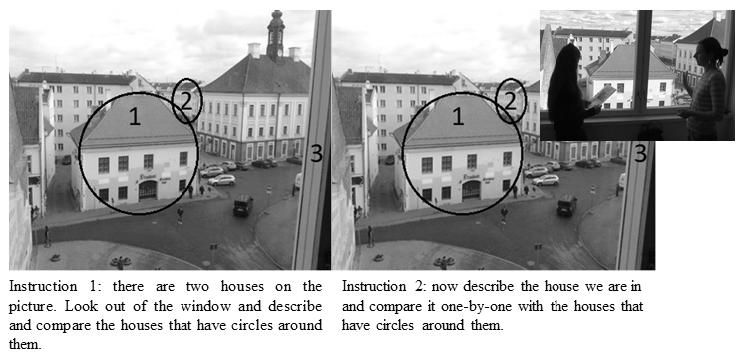
\includegraphics[width=\textwidth]{figures/a10Nahkolaetal20200422-img001.png}
\caption{The two-sided instruction sheet (The numbers are illustrative and were not included on the original instruction sheet.)}
\label{fig:nahkola:1}
\end{figure}

During the experiment, the experimenter stood next to the participant listening and giving minimal feedback. Resulting from the design of the task, the participants were operating with referents that were mutually known and identified – that is, presupposed (see \citealt{Silverstein1976}) by both interlocutors. The data contains a total of 86 monologues collected from 25 Russian, 33 Estonian and 28 Finnish native speakers. When citing the data, we give each example an individual code, which consists of an indicator of the language, an identifier of the speaker and a number identifying the referential unit.\footnote{For example, E14.027. E = Estonian, F = Finnish, R = Russian.}

The experiment consisted of two parts (Situation 1 and Situation 2). First, the participant described and compared two buildings, House 1 and House 2, of which House 1 was closer to the location of the participant and experimenter. In the second part, one more building (House 3) was added. This was the building where the participant and experimenter were located. By dividing the experiment into two parts, we were able to manipulate and observe the following factors: i) the change in the number of referents and thus the level of contrast, ii) the influence of distance and change in the deictic field. In addition to the aforementioned aspects, also other factors may influence the choice of the referential expression (for instance, the speaker’s psychological distance from the referent). In this study, however, we concentrate on the effect of distance and contrast.

The data analysed in this study contains the referential units that were used in the first part of the experiment (henceforth called Situation 1) to refer to the building close to the speaker (House 1). In other words, out of two competing referents, the focus is on the closer one. Focusing only on the closer referent enables us to distinguish spatially contrastive use from other discourse functions of the demonstratives in the data. We can be certain that the use of distal demonstrative adverbs in referring to House 1 is not due to the comparison of House 1 to the closest referent (as could be the case in Situation 2, when comparing House 1 to House 3). The decision to focus only on a subset of the data results in an analysis based on a relatively small amount of data. Therefore, our approach in the present study is qualitative and the quantitative data presented is only intended to show the proportional use of demonstrative adverbs and to point out tendencies in their usage. 

We have excluded from the analysis referential units that refer to only a part of a building. In some cases, the referential unit can refer to the location of the building or location inside the building instead of the building itself (see \sectref{sec:nahkola:4} for examples and discussion). In these cases, the speaker probably conceptualises the referent differently compared to the references that are concerning concrete features of the building (where the referent is conceptualised as an object). Nevertheless, we have included in our data also those referential units that refer to the referent’s location.

The experiments in all three languages were conducted and video-recorded at the same location in Tartu, Estonia. The recorded data was manually transcribed and annotated by native speakers. The transcription system employed was the Jefferson system \citep{Jefferson2004}. The data was annotated for a number of referential devices (see also \citealt{ReileEtAl2019}). For the present chapter, the most relevant categories are the first two mentioned and the last one on the list: demonstrative pronouns (in pronominal and adnominal use; later called BareDem and DemNP), demonstrative adverbs (DemAdv), NPs occurring without a demonstrative (BareNP), third person pronouns (PersPron), zero reference and different combinations of demonstrative pronouns, demonstrative adverbs and NPs. 

One more factor taken into account during the annotation of the data was the number of consecutive utterances in which the same referent was mentioned (that is, the tracking function of the referential unit). This factor, which henceforth is referred to as “mention number”, is related to the (dis)continuity of the referential chains formed by multiple references to the same entity. It is important to note that in this chapter, the term “first mention of the referent” does not indicate the absolute first time the referent is mentioned in the current discourse, but instead the first mention of the referent in the current referential chain. The annotation of the mention number enables us to explore the association between the information status of the referent and the choice of the referential expression. Following the terminology initiated by \citet{GundelEtAl1993,GundelEtAl2010}, we consider the first mention of the referential chain to comply with the status “familiar”. The subsequent mentions, in turn, comply with the statuses “in focus” and “activated”.

\section{Demonstratives in Russian, Estonian and Finnish}\label{sec:nahkola:3}

Estonian and Finnish as Finnic languages and Russian as a Slavic language have a three-directional system for demonstratives (goal, source and location). None of the languages makes a formal distinction between the demonstrative pronouns in their pronominal use and adnominal use (that is, as demonstrative determiners), but all three languages make a formal distinction between demonstrative pronouns and demonstrative adverbs. It should be noted, however, that in Finnish, the local cases of the demonstrative pronouns share some morphological, syntactic, and semantic features with the demonstrative adverbs. Therefore, the distinction between a demonstrative pronoun and an adverb is sometimes difficult to make in Finnish (see \sectref{sec:nahkola:3.3} and \citealt{Laury1996}). The demonstratives that are used for establishing a new referent are not formally distinguished from those that indicate a contrast between two already established referents. In Finnish and Estonian, demonstrative adverbs can be used adnominally, whereas in Russian this kind of use is not typically found. Estonian and Russian employ distance-based two-term systems; Finnish, in turn, has a mixed person- and distance-based system with three terms.

In the following sections, we present the most central features of the demonstrative systems in Russian, Estonian and Finnish.

\subsection{Russian demonstratives}\label{sec:nahkola:3.1}

There are two demonstrative pronouns – proximal \textit{eto} ‘this’ and distal \textit{to} ‘that’ – in contemporary Russian (\citealt[118]{Sheljakin2002}; \citealt[233]{Timberlake2004}). The spatial function of demonstratives activates mostly when two referents are in contrast; in other contexts, discourse factors are more important \citep{Grenoble1998}. Both have the same morphological stem (\textit{to}). In older Russian, the demonstrative \textit{se} was used for proximal reference, and this stem has been preserved in demonstrative adverbs up to the present.

Demonstrative adverbs are as follows: for location \textit{tut} ‘here’, \textit{zdes’} ‘here’ and \textit{tam} ‘there’; for goal \textit{sjuda} ‘to here’, \textit{tuda} ‘to there’; for source \textit{otsjuda} ‘from here’, \textit{ottuda} ‘from there’. Russian demonstrative adverbs do not normally co-occur with a noun phrase. There are some examples like \textit{tam, v nebesah} ‘there in the sky’ in written Russian, but the construction is better analysed as a case of apposition (see \citealt{Sahkai2003}) than as a single NP that contains a demonstrative adverb.

\textit{Tut} ‘here’ and \textit{zdes’} ‘here’ are both proximal demonstrative adverbs. \citet[105-106]{Grenoble1998} states that \textit{zdes’} indexes a concrete location – a physical space with dimension (\textit{Godami} \textit{on} \textit{rabotal} \textit{zdes’}. ‘For years he worked here [in the office]’). \textit{Zdes’} is used in opposition to \textit{tam} ‘there’. Moreover, when the ground is a concrete place, only \textit{zdes’} is acceptable. \textit{Tut} may also index a place when the place is an abstract space. The underlying opposition of ‘here’ to ‘there’, which is inherent to \textit{zdes’}, distinguishes it from \textit{tut}, which does not signal this opposition. Rather, \textit{tut} refers to a place with undetermined or irrelevant boundaries (\textit{Pochemu} \textit{ne} \textit{poznakomilsja} \textit{tut} \textit{ni} \textit{s} \textit{odnoj} \textit{iz} \textit{nih}? ‘Why haven’t you met a single one here [undefined space]?).

\subsection{Estonian demonstratives}\label{sec:nahkola:3.2}

Estonian has two demonstrative pronouns: \textit{see} ‘this’ and \textit{too} ‘that’. \textit{Too} has regionally varying use. In northern Estonia, \textit{too} is not used in spatial reference. In anaphoric reference, its use tends to be restricted to time expressions and in reference to the second human character of a literary narrative \citep{Pajusalu2006}. Therefore, based on spatial distinctions made by demonstrative pronouns, Estonian has two demonstrative pronoun systems: a one-term system, where \textit{see} ‘this/that’ is distance-neutral \citep{Reile2015,Pajusalu2009} and a two-term system, where \textit{see} ‘this’ is the proximal and \textit{too} ‘that’ the distal demonstrative pronoun \citep{Reile2016}. In addition, both demonstrative pronouns can be used as definite determiners but \textit{see} is used much more frequently in this function \citep{Pajusalu2009}. Moreover, the demonstrative pronoun \textit{see} and third person pronoun \textit{tema/ta} share the anaphoric referential domain. In addition, both of these pronouns can be used to refer to animate and inanimate referents depending on their activation status \citep{Pajusalu2017}.

Estonian has six demonstrative adverbs displaying two distance-based contrasts, goal-based \textit{siia} ‘hither’ and \textit{sinna} ‘thither’, location-based \textit{siin} ‘here’ and \textit{seal} ‘there’, and source-based \textit{siit} ‘from here’ and \textit{sealt} ‘from there’. In spatial reference, \textit{siin} ‘here’ is the proximal and \textit{seal} ‘there’ is the distal demonstrative adverb. Demonstrative adverbs can also be used as definite determiners in place denoting NPs (e.g. \textit{seal} \textit{majas} ‘(in) yonder house’). Moreover, distal demonstrative adverbs can be used to denote previously mentioned location in a narrative \citep{Pajusalu2017}.

\subsection{Finnish demonstratives}\label{sec:nahkola:3.3}

The Finnish language has three demonstrative pronouns: \textit{tämä/tää} ‘this’, \textit{tuo/ toi} ‘that’ and \textit{se} ‘it, that, the’.\footnote{\textit{Tämä} and \textit{tuo} are used in standard Finnish, \textit{tää} and \textit{toi} in many colloquial varieties.} According to the traditional, largely distance-based view (e.g. \citealt{Larjavaara1990}), \textit{tämä} ‘this’ refers to a referent near the speaker and \textit{tuo} ‘that’ to a referent distant from both the speaker and the addressee. This view is not entirely based on distance, as it considers \textit{se} ‘it, that, the’ to be distance-neutral. Moreover, \textit{se} is hearer-centred, whereas \textit{tämä} and \textit{tuo} are speaker-centred. However, several accounts \citep{Itkonen1966,Laury1997,Seppänen1998,Etelämäki2006} have proposed an analysis relying more on the social and interactional functions of the Finnish demonstratives.

In addition to its hearer-centred meaning, \textit{se} functions as an anaphoric device, maintaining reference when the referent is already activated and sufficiently defined \citep{Laury1997,Etelämäki2005,Duvallon2005}. \textit{Se} can also identify a referent that is considered to be known in advance \citep{Laury1997}. \textit{Tämä} and \textit{tuo} are primarily exophoric \citep{HakulinenEtAl2004}, but can also be used anaphorically. Anaphoric \textit{tämä} and \textit{tuo} indicate a higher level of salience for the referent than \textit{se}. Moreover, \textit{tämä} and \textit{tuo} indicate open reference – in other words, they imply that the process of identifying the referent is still ongoing. \textit{Se}, on the other hand, marks closed reference \citep{Etelämäki2005}. \textit{Tuo} has also been reported to show a speaker’s dissociation or uncertainty in relation to a referent \citep{Hakulinen1985,Laury1997}.

Finnish demonstrative adverbs share the same three-stem system with demonstrative pronouns. Demonstrative pronouns inflect for most Finnish cases, including for six cases that indicate a place of action. These local cases are divided into two groups according to whether the action takes place inside a three-dimensional location (internal cases) or outside or on a two-dimensional location (external cases) \citep{HakulinenEtAl2004}. The locative demonstrative adverbs have only three forms: location, source and goal. Only pronouns have plural forms, but adverbs can co-occur with a noun which is in plural form. The paradigms of the local case forms of the pronouns and the demonstrative adverbs partially overlap. All (singular) forms are presented in \tabref{tab:nahkola:1}.\footnote{The brackets indicate the parts that are often omitted in spoken language, for example \textit{tuonne} > \textit{tonne}. In addition, the suffixal parts of the demonstratives are often shortened, e.g. \textit{täällä} > \textit{tääl,} \textit{siinä} > \textit{siin}.}

%Adjust table formatting, check: should language data been in italics?
\begin{table}
\begin{tabularx}{\textwidth}{QQQQ}
\lsptoprule
{Demonstrative stems} & {Adverbs} & {Internal case forms of the pronouns} & {External case forms of the pronouns}\\
\midrule
{tä-} & {täällä, täältä, tänne} & {tässä, tästä, tähän} & {tällä, tältä, tälle}\\
\tablevspace
{t(u)o-} & {tuolla, tuolta, t(u)onne} & t(u)ossa, t(u)osta, t(u)ohon & t(u)olla, t(u)olta, t(u)olle\\
\tablevspace
{se-} & {siellä, sieltä, sinne} & {siinä, siitä, siihen} & {sillä, siltä, sille}\\
\lspbottomrule
\end{tabularx}
\caption{Spatial demonstratives in Finnish (location, source, goal)}
\label{tab:nahkola:1}
\end{table}

There is not full agreement on the categorisation of the Finnish spatial demonstratives (see \citealt{Laury1996} for an overview of the discussion). \citet{Laury1996} suggests treating the local demonstratives as a continuum, where the adverbs are the most adverbial and the external case forms the least adverbial forms. The label “the least adverbial” refers to the syntactic and semantic features of the external cases: in actual speech, they are primarily used to express non-locative functions – for example, possessor or recipient – and only occasionally refer to locations \citep{Laury1996,Laury1997}. In addition, they always behave syntactically like pronouns. The internal local cases, in turn, can manifest an adverb-like behaviour. In this study, the term “internal local cases” refers to these locative forms of the pronouns that carry also adverb-like features.

Both demonstrative adverbs and demonstrative pronouns can be used adnominally \citep{HakulinenEtAl2004}. When occurring with a noun, the pronouns tend to agree with the head of the noun phrase in both case and number, whereas the adverbs do not. Similar to adverbs, the internal case forms of demonstrative pronouns do not always agree with the head of the noun phrase. Moreover, the internal cases can co-occur with an adverb or a postpositional phrase, unlike other pronouns. How then do speakers make choices between pronominal and adverbial demonstratives in spatial reference in Finnish? For example, the following factors have been suggested to affect the choice between the forms: exactness of reference, visibility of the referent, proximity of the referent and the size or the boundedness of the referenced area (e.g. \citealt{Itkonen1966,Siitonen1979,Östman1995}).\footnote{In addition to the aforementioned authors, \citet{Laury1996} proposes an interesting analysis based on the conceptualisation of scenes in terms of figure and ground (see also \citealt{Talmy1983}). The referents referred to with internal cases tend to be conceptualised as figures and the ones referred to with adverbs as grounds.}

Even though the internal local case forms of pronouns resemble adverbs in many ways, the internal cases are not always used to indicate location. Like the external case forms, the internal cases can express non-local concepts such as a part–whole relationship or physical/mental state. Adverbs, on the other hand, do not express any concepts other than concrete location (at least in our data).

\section{Results}\label{sec:nahkola:4}

In the present analysis, the focus is on referential units referring to the proximal building (House 1) during the first part of the experiment (Situation 1). The focus of the analysis is on demonstrative adverbs, but we will begin by giving an overview of all referential devices that are used to refer to House 1 in Situation 1 (see \tabref{tab:nahkola:2}).

%adjust table formatting
\begin{table}
\small
\begin{tabularx}{\textwidth}{Xrrrrrr}
\lsptoprule
\multicolumn{2}{l}{Language} & \multicolumn{4}{c}{{Referential device}}\\
\cmidrule{2-6}
 & {BareDem} & {DemNP} & {BareNP} & {PersPron} & {Zero} & {Total}\\
 \midrule
{RUS} & {47 (17\%)} & {29 (10.5\%)} & {113 (40.9\%)} & {68 (24.6\%)} & {19 (6.9\%)} & {276 (100\%)}\\
{EST} & {74 (18.6\%)} & {89 (22.4\%)} & {177 (44.6\%)} & {45 (11.3\%)} & {12 (3\%)} & {397 (100\%)}\\
{FIN} & {218 (57.1\%)} & {113 (29.6\%)} & {45 (11.8\%)} & {$-$} & {6 (1.6\%)} & {382 (100\%)}\\
\lspbottomrule
\end{tabularx}
\caption{\label{tab:nahkola:2}
All referential units referring to House 1 in Situation 1 (BareDem = demonstrative (pronoun or adverb) without a separate nominal head; DemNP = demonstrative (pronoun or adverb) with a separate nominal head; BareNP = noun phrase without a demonstrative; PersPron = third person pronoun; Zero = zero reference)}
\end{table}

The most striking differences between the data from the three languages are the following: i) the proportion of referential units that include a demonstrative is larger in the Finnish data than in the data for the other two languages; this is especially true for the bare demonstratives (that is, the demonstratives without a head noun); ii) conversely, Finnish has the smallest number of referential units that do not include a demonstrative (BareNP). Moreover, Finnish does not employ personal pronouns for inanimate referents, whereas in the Russian data personal pronouns are the second most frequent referential device. In most of the categories (nominal and adnominal demonstratives, personal pronouns and zero reference) presented in \tabref{tab:nahkola:2}, Estonian is situated between Finnish and Russian when it comes to the frequency of different referential devices. The proportion of the referential units made up of bare NPs is, however, the largest in the Estonian data.

Next, we will describe the use of demonstrative adverbs in the three languages (see \tabref{tab:nahkola:3}).

\begin{table}
\begin{tabularx}{\textwidth}{lrrYr}
\lsptoprule
{Language} & \multicolumn{3}{c}{{Demonstrative adverb}} & {Total}\\
\cmidrule{2-4}
& {Proximal} & {Distal} & {Hearer-centred{\slash}Anaphoric} & \\
\midrule
{RUS} & {15 (44.1\%)} & {19 (55.9\%)} & {$-$} & {34 (100\%)}\\
{EST} & {33 (62.3\%)} & {20 (37.7\%)} & {$-$} & {53 (100\%)}\\
{FIN} & {1 (5.0\%)} & {4 (20.0\%)} & {15 (75.0\%)} & {20 (100\%)}\\
\lspbottomrule
\end{tabularx}
\caption{Demonstrative adverbs referring to House 1 in Situation 1}
\label{tab:nahkola:3}
\end{table}

Although Finnish has the greatest number of referential units with a demonstrative, it has the smallest number of units with a demonstrative adverb.\footnote{It should be noted that also the internal local cases of Finnish demonstrative pronouns exhibit adverb-like behaviour. These forms are not included in \tabref{tab:nahkola:3}. Instead, we discuss the use of the internal local cases in \sectref{sec:nahkola:4.3}.} The Estonian data includes more demonstrative adverbs than the Russian data, which is in line with the overall frequency of demonstratives in both languages (presented above in \tabref{tab:nahkola:2}). In the Russian data, distal adverb forms are the most frequent, unlike in the Estonian data, where proximal forms outnumber distal forms. The Finnish data includes mostly hearer-centred/anaphoric demonstrative adverbs. In this context, only the anaphoric function is relevant, as the referent is at the same distance from both interlocutors. The hearer-centred function activates only in situations where the addressee’s current sphere is conceived as distinct from the speaker’s sphere (see \citealt{Larjavaara1985}).

We will discuss the data for each language more thoroughly in the following sections. 

\subsection{The use of demonstrative adverbs in the Russian data}\label{sec:nahkola:4.1}

In the Russian data for House 1 in Situation 1, there are a total of 34 referential units with demonstrative adverbs, 15 proximal (14 \textit{zdes’} ‘here’, 1 \textit{tut} ‘here’) and 19 distal (\textit{tam} ‘there’) (see \tabref{tab:nahkola:4}). In the Russian data, demonstrative adverbs do not function as determiners.

\begin{table}
\begin{tabularx}{\textwidth}{Xrrrr}
\lsptoprule
{Adverbs} & {1\textsuperscript{st} mention} & {2\textsuperscript{nd} mention} & {3\textsuperscript{rd} mention and further} & {Total}\\
\midrule
{tut/zdes’} & {9 (60.0\%)} & {5 (33.3\%)} & {1 (6.7\%)} & {15 (100\%)}\\
{tam} & $-$ & {7 (36.8\%)} & {12 (63.2\%)} & {19 (100\%)}\\
\lspbottomrule
\end{tabularx}
\caption{The use of Russian demonstrative adverbs in referring to House 1 in Situation 1}
\label{tab:nahkola:4}
\end{table}

\textit{Zdes’} and \textit{tut} always refer to House 1 in Situation 1, see \REF{ex:nahkola:1} and \REF{ex:nahkola:2}. Distal \textit{tam} refers mostly to House 2, but sometimes also to House 1, see \REF{ex:nahkola:3}. This, in addition to the fact that \textit{tam} is not used for first mentions in the referential chain, suggests that in addition to indicating distance, \textit{tam} can function as an anaphoric device. When \textit{tam} is used anaphorically, the contrast between the referents is not relevant.


\ea\label{ex:nahkola:1} (R20.041)\footnote{See the appendix for a list of symbols used in the transcription.}\\
{a (.) {трубы} (.) {по} {которым} {стекает} {вода}, \textbf{{здесь}} {я} {их} {вижу} {на} {каждом} {уголку}, {они} {стоят} (.) {висят}. a \textbf{{там} (.) {там}} {я} {вообще} {их} {не} {вижу}.} \\
\gll a, truby, po kotorym stekaet voda, \textbf{zdes’} ja ih vizhu na kazhdom ugolku, oni stojat, visjat. a \textbf{tam,} \textbf{tam} ja voobsche ih ne vizhu. \\
     o pipe.\textsc{pl} \textsc{prep} \textsc{rel} flow.down.\textsc{3sg} water.\textsc{nom} here \textsc{1sg} \textsc{3pl.acc} see.\textsc{1sg} \textsc{prep} every\textsc{.loc} corner.\textsc{dim.loc} \textsc{3pl} stand.\textsc{3pl} hang.\textsc{3pl} but there there \textsc{1sg} at.all \textsc{3pl} \textsc{neg} see.\textsc{1sg}\\
\glt ‘O, pipes in which water flows down, \textbf{here} I can see them on every corner, they are standing, hanging. But \textbf{there,} \textbf{there} I can’t see them at all.’ 
\z

\ea\label{ex:nahkola:2} (R06.061)\\
{... \textbf{{тут}} {написано ресторан-бар.}}\\
\gll ... \textbf{tut} napisano {restoran bar}.\\
     {} here.\textsc{dem.adv.loc} write.\textsc{perf.ptcp} restaurant.bar.\textsc{nom}\\
\glt ‘\textbf{Here} it says “restaurant-bar”.’ 
\z

\ea\label{ex:nahkola:3} (R22.007)\footnote{The preceding context for the example is the following: {вот, в принципе здание небольшое. эх, что ещё можно сказать? много окон. так же я думаю там два входа, если я не ошибаюсь.} ‘So practically it is not a big building. Oh, what else could I say? Lots of windows. I also think there are two entrances, if I am not wrong.’}\\
{{так} {же} {я} {думаю} \textbf{{там}} {два} {входа},} \\
\gll tak zhe ja dumaju \textbf{tam} dva vhoda,\\
     also \textsc{prtcl} \textsc{1sg} think.\textsc{1sg} there.\textsc{dem.adv.loc} two entrance.\textsc{gen}\\
\glt ‘Also, I think there are two entrances \textbf{there}.’ 
\z

While the usage contexts of \textit{tam} are mostly different from the contexts typical for the other two demonstrative adverbs, it is more difficult to pinpoint the differences between the adverbs \textit{zdes’} and \textit{tut}. However, some tendencies can be detected. In this part of the analysis, we take into account the data concerning both House 1 and House 3 (the building where the interlocutors are located). This enables us to provide a more comprehensive account of the usage contexts of the two proximal adverbs. Firstly, 83\% (n=10) of the occurrences of \textit{tut} refer to House 3, whereas with \textit{zdes’}, the proportion of the units referring to House 3 is smaller (64\%, n=27). Consequently, \textit{zdes’} is used to refer to House 1 more often than \textit{tut} (\textit{zdes’} 36\%, n=15; \textit{tut} 17\%, n=2). Secondly, the analysis regarding the mention numbers of the referential units reveals another difference between the usage patterns of these two adverbs. 75\% (n=9) of the referential units containing \textit{tut} are the first mentions of the referential chain, whereas with \textit{zdes’}, the proportion of first mentions is 48\% (n=20). To conclude, our data suggests that the main function of \textit{zdes’} is contrastive and \textit{zdes’} is less often used for identifying a referent at first mention than \textit{tut}. In our context, \textit{tut} seems to specialise for House 3, which is the location of the interlocutors. As the boundaries of House 3 are not observable for the speaker, this building is conceptualised as space, while House 1, which can be seen through a window, is conceptualised as an object. This supports \citegen{Grenoble1998} finding discussed in \sectref{sec:nahkola:3.1}: \textit{zdes’} indexes a concrete location and is used in opposition to \textit{tam} ‘there’, while \textit{tut} refers to a place with undetermined or irrelevant boundaries.

\subsection{The use of demonstrative adverbs in the Estonian data}\label{sec:nahkola:4.2}

In the Estonian data for House 1 in Situation 1, \textit{siin} ‘here’ is used 33 times and \textit{seal} ‘there’ 20 times. The analysis of the mention number of the referential unit reveals that the use of \textit{seal} increases and \textit{siin} decreases as the mention number increases (see \tabref{tab:nahkola:5}). This suggests that in our data, the majority of the referential units with \textit{siin} are used spatially \REF{ex:nahkola:4}, whereas \textit{seal} is used mostly anaphorically \REF{ex:nahkola:5}. However, the anaphoric use of \textit{siin} is also possible \REF{ex:nahkola:6}.

\begin{table}
\begin{tabularx}{\textwidth}{XrrYr}
\lsptoprule
{Demonstrative adverb} & {1\textsuperscript{st} mention} & {2\textsuperscript{nd} mention} & {3\textsuperscript{rd} mention and further} & {Total}\\
\midrule
{\textit{siin}} & {19 (57.6\%)} & {11 (33.3\%)} & {3 (9.1\%)} & {33 (100\%)}\\
{\textit{seal}} & {3 (15.0\%)} & {3 (15.0\%)} & {14 (70.0\%)} & {20 (100\%)}\\
\lspbottomrule
\end{tabularx}
\caption{The use of Estonian demonstrative adverbs in referring to House 1 in Situation 1}
\label{tab:nahkola:5}
\end{table}

\ea\label{ex:nahkola:4} (E15.003)\\
\gll \textbf{sellel} \textbf{majal} \textbf{siin} on (.) selline uhke silmatorkav katus ...\\
     this.\textsc{dem.pron.ade} house.\textsc{ade} here.\textsc{dem.adv.loc} be.\textsc{prs.3sg} {} this.kind.\textsc{nom} grand.\textsc{nom} conspicuous.\textsc{nom} roof.\textsc{nom}\\
\glt ‘\textbf{This} \textbf{house} \textbf{here} has a grand roof ...’ 
\z

\ea\label{ex:nahkola:5} (E17.001; E17.003; E17.004)\\
\gll nii \textbf{esimesel} \textbf{majal} on selline pruunikas punane katus? (.) \textbf{üsna} \textbf{vana} \textbf{maja} tundub olema, ilmselt on \textbf{seal} olnud mingi restoran või baar,\\
     so first.\textsc{ade} house.\textsc{ade} be.\textsc{prs.3sg} this.kind.\textsc{nom} brown.\textsc{nom} red.\textsc{nom} roof.\textsc{nom} {} rather old.\textsc{nom} house.\textsc{nom} seem.\textsc{prs.3sg} be.\textsc{inf} apparently be.\textsc{prs.3sg} there.\textsc{dem.adv.loc} be.\textsc{pst.ptcp} some.kind restaurant.\textsc{nom} or bar.\textsc{nom}\\
\glt ‘(The) \textbf{first} \textbf{house} has a brownish red roof. (It) looks like \textbf{quite} \textbf{an} \textbf{old} \textbf{house}, \textbf{there} has probably been a restaurant or bar.’ 
\z

\ea\label{ex:nahkola:6} (E01.051; E01.052)\\
\gll \textbf{esimene} \textbf{maja} on väljast väga hästi valgustatud \textbf{siin} on lausa päris mitu valgustit ees ...\\
     first.\textsc{nom} house.\textsc{nom} be.\textsc{prs.3sg} outside.\textsc{ela} very well light.\textsc{pst.ptcp} here.\textsc{dem.adv.loc} be.\textsc{prs.3sg} even quite many lamp.\textsc{part.pl} in.front\\
\glt ‘\textbf{The} \textbf{first} \textbf{house} is very well lit, there are many lights \textbf{here} ...’ 
\z

When the speaker refers to House 1 in Situation 1 with \textit{seal}, the same referent has usually been mentioned in the previous utterance and is in the current focus of attention \REF{ex:nahkola:5}.

Estonian demonstrative adverbs can be combined with NPs and demonstrative pronouns \REF{ex:nahkola:4}. While in general \textit{see} ‘this’ can occur with both distal \textit{seal} and proximal \textit{siin}, \textit{too} ‘that’ seems to be combined only with distal \textit{seal} (e.g. \citealt{Reile2016}). However, in the current data, \textit{see} occurs only with proximal \textit{siin.}\footnote{There were no instances of \textit{too} used in reference to House 1 and therefore also no combinations with the adverbs.} The compound forms are used mostly, but not always, for the first mention of the referent in the referential chain.

The adverb \textit{siin} usually comes after the pronoun \textit{see} (and possible NP) in the utterance \REF{ex:nahkola:7}.

\ea\label{ex:nahkola:7} (E30.031; E30.033)\\
\gll siin ei tea mis seal katuse all on (...) \textbf{see} \textbf{siin} jah? on tänavale ka rohkem avatud (.) kuna autod sõidavad mööda ...\\
     here.\textsc{dem.adv.loc} \textsc{neg} know.\textsc{prs}.1\textsc{sg} what there.\textsc{dem.adv.loc} roof.\textsc{gen} under be.\textsc{prs.3sg} {} this.\textsc{dem.pron.nom} here.\textsc{dem.adv.loc} yes be.\textsc{prs.3sg} street.\textsc{all} also more open {} since car.\textsc{pl.nom} drive.\textsc{prs.3pl} by\\
\glt ‘Here I don’t know what is under the roof (up) there. \textbf{This} \textbf{here} is more open to the street as well since the cars drive by …’ 
\z

\textit{Siin} can also occur before \textit{see} \REF{ex:nahkola:8}, but the occurrence of \textit{siin} in this position is very rare in our data (only one use for House 1 in Situation 1).

\ea\label{ex:nahkola:8} (E31.020)
\gll sellel tagumisel on katuseaknad aga \textbf{siin} \textbf{sellel} \textbf{esimesel} \textbf{majal} ei ole katuseaknaid,\\
     this.\textsc{dem.pron.ade} hindmost.\textsc{ade} be.\textsc{prs.3sg} skylight.\textsc{nom.pl} but here.\textsc{dem.adv.loc} this.\textsc{dem.pron.ade} first.\textsc{ade} house.\textsc{ade} \textsc{neg} be skylight.\textsc{nom.pl}\\
\glt ‘This one at the back has skylights but \textbf{here} \textbf{this} \textbf{house} \textbf{in} \textbf{the} \textbf{front} does not have skylights.’ 
\z

In \REF{ex:nahkola:8}, where \textit{siin} occurs before \textit{see}, the referential unit is the first mention of the referent in the current referential chain and the referent is not in focus. The speaker uses \textit{siin} to define the visual region in which the addressee should look for the referent, and then identifies the house by using a demonstrative pronoun and a lexical NP (\textit{sellel esimesel majal}). In \REF{ex:nahkola:7} where\textit{ siin} comes after \textit{see}, the house has been mentioned in the previous utterance and is in the current focus of attention. This pattern of demonstrative adverb use suggests that in Estonian, the position of demonstrative adverbs in a referential utterance can be used to connect the visual world with the cognitive status of the referent and through this to indicate whether or not the referent is in the current joint focus of attention of the interlocutors. This is in line with previous findings regarding the use of Estonian demonstrative adverbs for spatial reference \citep{Reile2015,Reile2016}.

In our data, when referring to the buildings, Estonian speakers also use demonstrative pronouns and third person pronouns – which are common anaphoric devices in Estonian \citep{Pajusalu2009}. In Estonian, both demonstrative adverbs and demonstrative pronouns occur as determiners in place-denoting NPs. While demonstrative pronouns and third person pronouns can occur in any case form, internal case forms are central to the current study. More specifically, the case form that is most of interest is the inessive (an internal case form), e.g. \textit{selle-s maja-s} ‘in this/that house’, where -\textit{s} is the inessive case marker. The alternative referential devices that could be used instead of a pronoun in the inessive case are the demonstrative adverbs. However, since demonstrative adverbs can occur with demonstrative pronouns, these referential devices can also complement each other, instead of being only alternative devices.

To conclude, the proximal demonstrative adverb \textit{siin} is used mainly spatially and the distal demonstrative adverb \textit{seal} is used anaphorically when referring to House 1 in Situation 1. The longer the referential chain, the more instances of distal \textit{seal} and the fewer of proximal \textit{siin} occur. Out of the two demonstrative adverbs in Estonian, only \textit{siin} occurs in demonstrative pronoun and adverb combinations in our data. By combining demonstrative pronouns and demonstrative adverbs in the same referential unit, the speaker can provide information on the referent at different levels of discourse as well as double the force of the spatial reference.

\subsection{The use of demonstrative adverbs in the Finnish data}\label{sec:nahkola:4.3}

In the Finnish data, demonstrative adverbs are used for referring to House 1 a total of 20 times in Situation 1 (see \tabref{tab:nahkola:6}). If we also consider the use of the internal case forms of demonstrative pronouns (presented later in \tabref{tab:nahkola:7}), this number increases to 102. In the present analysis, the internal local cases of the Finnish demonstrative pronouns are taken into account when they appear without a head noun \REF{ex:nahkola:9}.

\ea\label{ex:nahkola:9} (F15.014)\\
\gll \textbf{täs} on tietysti vaan (.) ravintola ja baari?\\
     this.\textsc{dem.pron.ine} be.\textsc{prs.3sg} of.course only {} restaurant.\textsc{nom} and bar.\textsc{nom}\\
\glt ‘\textbf{Here} is, of course, just a restaurant and a bar.’ 
\z

The internal local cases of pronouns are analysed separately from the adverbs due to their somewhat different usage patterns. Therefore, we have excluded from the present analysis the forms that cannot be unambiguously placed into either the adverb or pronoun category. This means that internal case forms occurring in the same case as a head noun, like in \REF{ex:nahkola:10}, are excluded.\footnote{Example 10 epitomises the difficulties of differentiating between the pronominal and adverbial uses of the internal case forms. Following the criteria given in \sectref{sec:nahkola:3.3}, the demonstrative \textit{tässä} is unambiguously a pronoun, since it agrees with the head of the phrase in case and number. However, one could argue that \textit{tässä} is external to the phrase and just happens to occur in the same case with \textit{lähemmässä} \textit{talossa}. The pause between \textit{tässä} and \textit{lähemmässä} \textit{talossa} could point to such an analysis (see \citealt[86]{Laury1996} for a similar discussion). Nevertheless, \REF{ex:nahkola:10} and others like it are not included in the present analysis.}

\ea\label{ex:nahkola:10} (F28.051)\\
\gll \textbf{tässä} (.) \textbf{lähemmässä} \textbf{talossa} on myös tollaset isot (.) valot?\\
     this.\textsc{dem.pron.ine} {} near.\textsc{comp.ine} house.\textsc{ine} be.\textsc{prs.3sg} also such\textsc{.nom.pl} light.\textsc{nom.pl} {} big.\textsc{nom.pl}\\
\glt ‘\textbf{In} \textbf{this} \textbf{nearer} \textbf{house}, there are also those big lights.’
\z

The external case forms of the demonstrative pronouns are not included in the analysis, since their adverb-like use is not found in our data and their frequency is low.\footnote{For comparison: the external case forms are used to refer to the buildings a total of 8 times in our data (and none of these uses expresses location), whereas the internal case forms are used 335 times.} 

In our discussion, first, we focus on the demonstrative adverbs only. Then, we discuss the use of the internal local cases in comparison with the use of the demonstrative adverbs.

\begin{table}
\begin{tabularx}{\textwidth}{XrrYr}
\lsptoprule
{DemAdv stem} & {1\textsuperscript{st} mention} & {2\textsuperscript{nd} mention} & {3\textsuperscript{rd} mention and further} & {Total}\\
\midrule
{tää-} & – & – & {1 (100\%)} & {1 (100\%)}\\
{t(u)o-} & {1 (25.0\%)} & – & {3 (75.0\%)} & {4 (100\%)}\\
{se-} & – & {4 (26.7\%)} & {11 (73.3\%)} & {15 (100\%)}\\
\lspbottomrule
\end{tabularx}
\caption{The use of Finnish demonstrative adverbs in referring to House 1 in Situation 1}
\label{tab:nahkola:6}
\end{table}

The speakers refer to House 1 with demonstrative adverbs mostly when the referent has already been mentioned in one or more previous utterances. The most frequent stem is the hearer-centred/anaphoric \textit{se}-stem.\footnote{\textit{Se}-stem has also two other variants (\textit{sie}- and \textit{sii}-) but for clarity they are also referred to as \textit{se}-stem.} This is in line with the previous findings showing that \textit{se-}stem demonstratives are used for referents that are activated and already sufficiently identified \citep{Laury1997,Etelämäki2006}. In our Finnish data related to House 1, the demonstrative adverbs are used mostly for maintaining the reference while the main function of the utterance is related to something else than identifying the referent. It can be, for instance, describing details of the referent like in \REF{ex:nahkola:11}. Here, the same building (House 1) has been mentioned in several preceding utterances, as the speaker has been describing its roof. The speaker is using the demonstrative adverb \textit{siellä} ‘(in) there’, which has the most common anaphoric stem.

\ea\label{ex:nahkola:11} (F07.011)\footnote{The preceding context for the example is the following: \textit{jos} \textit{mun} \textit{pitäisi} \textit{kuvailla} \textit{sitä} \textit{ihmiselle} \textit{joka} \textit{ei} \textit{näe} \textit{sitä} \textit{niin} \textit{se} \textit{on} \textit{sanoisin} \textit{että} (.) \textit{se} \textit{on} \textit{ensin} \textit{hyvin} \textit{suorakulmainen,} \textit{melkein} \textit{neliö}. ‘If I needed to describe it to a person who does not see it, then it is, I would say that at first it is very rectangular, almost like a square.’}\\
\gll ja \textbf{siellä} on kaunis kolmiomainen kartiomainen (.) tiilikatto? joka on minusta aina ollut (.) {kaunein kattoma(lli)}.\\
     and there.\textsc{dem.adv.loc} be.\textsc{prs.3sg} beautiful.\textsc{nom} triangular.\textsc{nom} conical.\textsc{nom} {} brick.roof.\textsc{nom} that be.\textsc{prs.3sg1sg.ela} always be.\textsc{pst.ptcp} beautiful.\textsc{supl.nom} {} roof.type.\textsc{nom}\\
\glt ‘And there is a beautiful triangular (or) conical brick roof \textbf{there}, which I have always thought to be the most beautiful roof ty(pe).’ 
\z

Next, we will examine the use of internal local cases when referring to House 1, see \tabref{tab:nahkola:7} and \REF{ex:nahkola:9}.

\begin{table}
\begin{tabularx}{\textwidth}{XrrYr}
\lsptoprule
{DemPron stem} & {1\textsuperscript{st} mention} & {2\textsuperscript{nd} mention} & {3\textsuperscript{rd} mention and further} & {Total}\\
\midrule
{tä-} & {23 (76.7\%)} & {4 (13.3\%)} & {3 (10\%)} & {30 (100\%)}\\
{t(u)o-} & {5 (71.4\%)} & {2 (28.6\%)} & – & {7 (100\%)}\\
{se-} & {2 (4.4\%)} & {12 (26.7\%)} & {31 (68.9\%)} & {45 (100\%)}\\
\lspbottomrule
\end{tabularx}
\caption{The use of the internal local cases of demonstrative pronouns in referring to House 1 in Situation 1}
\label{tab:nahkola:7}
\end{table}

Compared to the data on the demonstrative adverbs above, the data on the use of internal local cases reveals somewhat different referential practices. Internal local cases are used for first mentions (in the referential chain) more often than adverbs. Since there are more first mentions, there are also more \textit{tä}- and \textit{t(u)o}-stems, as these stems are used for identifying a referent and they typically indicate that the process of identifying the referent is unfinished \citep{Laury1997,Etelämäki2005}. Similar to adverbs, the \textit{se}-stem is the most frequently used stem also among the pronouns.

Demonstrative adverbs can co-occur with demonstrative pronouns in compound forms. Typically, both demonstratives in a compound form have the same stem, but also compounds containing demonstratives with different stems are possible. The frequency of compound forms is low in the Finnish data (a total of 16 referential units in the data, including all referents and both parts of the experiment). Therefore, in this part of the analysis, we will use examples concerning all three referents (Houses 1, 2 and 3). The most typical structure of a demonstrative compound is either pronoun+adverb \REF{ex:nahkola:12} or pronoun+noun+adverb \REF{ex:nahkola:13}. It is also possible for the adverb to precede the pronoun.

\ea\label{ex:nahkola:12} (F21.031)\\
\gll ja (.) draakkonin rakennus on pienempi ku \textbf{toi} (.) \textbf{toi} \textbf{tuolla}.\\
     and {} draakkon.\textsc{gen} building.\textsc{nom} be.\textsc{prs.3sg} small.\textsc{comp.nom} than that.\textsc{dem.pron.nom} {} that.\textsc{dem.pron.nom} over.there.\textsc{dem.adv.loc}\\
\glt ‘And the Draakkoni building is smaller than \textbf{that} \textbf{one} \textbf{over} \textbf{there}.’ 
\z

\ea\label{ex:nahkola:13} (F19.001)\\
\gll no: tää on luultavasti vanhempi \textbf{tää} (.) \textbf{draakkoni} \textbf{tässä},\\
     well this.\textsc{dem.pron.nom} be.\textsc{prs.3sg} probably old.\textsc{comp.nom} this.\textsc{dem.pron.nom} {} draakkoni.\textsc{nom} this.\textsc{dem.pron.ine}\\
\glt ‘Well this one is probably older, \textbf{this} \textbf{Draakkoni} (= name of the building) \textbf{here}.’ 
\z

When internal local cases of pronouns appear in compound forms, their adverb-like features are particularly apparent. Unlike other pronouns, internal local cases of demonstratives can appear after the head of the noun phrase, as in \REF{ex:nahkola:13} above, where the demonstrative pronoun \textit{tässä} appears in a position which is typical for adverbs in compound forms.

The co-occurrence of two demonstratives reinforces the pragmatic function of the referential unit \citep[474]{Diessel2006}. The speaker’s motivation to use a compound form can connect to hesitation and uncertainty about whether the intended referent has been sufficiently identified in order to be distinguished from the competing referents. The pauses inside the referential units in \REF{ex:nahkola:12} and \REF{ex:nahkola:13} could also point in this direction, as well as the dislocated position of the referential unit containing the compound form in \REF{ex:nahkola:13} (on the role of right-dislocations in reducing disambiguation and clarifying the referent, see e.g. \citealt{Geluykens1987}).

Both the adverbs and the internal case forms can be used for identifying a referent and tracking a referent. By choosing either the adverbial form or the pronominal form of a demonstrative, the speaker can emphasise certain features of the referent. In \REF{ex:nahkola:14}, the speaker first refers to House 2 (the more distant building) with a distal adverb \textit{tuol} (‘over there’). Then follows a reference to House 1 (the closer building) by using the same distal stem but this time in a pronominal form (\textit{tos} ‘in that’). At this point, the contrast between the two referents is formed by using an adverb for one and a pronoun for the other referent. At the end of the utterance, the speaker refers to House 1 once more with an expression that contains an NP with a demonstrative pronoun, this time with a proximal stem (\textit{tässä} ‘in this’).

\ea\label{ex:nahkola:14} (F21.015)\\
\gll (.) noi ei oo savupiiput ku \textbf{tuol}= on mut \textbf{tos}= on vanha savupiippu \textbf{tässä} \textbf{draakkonis}.\\
     {} that.\textsc{dem.pron.nom.pl} \textsc{neg} be.\textsc{prs.3sg} chimney.\textsc{nom.pl} that over.there.\textsc{dem.adv.loc} be.\textsc{prs.3sg} but that.\textsc{dem.pron.ine} be.\textsc{prs.3sg} old.\textsc{nom} chimney.\textsc{nom} this.\textsc{dem.pron.ine} draakkon.\textsc{ine}\\
\glt ‘Those \textbf{over} \textbf{there} are not chimneys, but \textbf{that} \textbf{one} has an old chimney, \textbf{this} \textbf{Draakoni}.’ 
\z

Keeping in mind the list of possible factors affecting the choice of the referential device (exactness of reference, visibility of the referent, proximity of the referent and the size or the boundedness of the area referred to; see \sectref{sec:nahkola:3.3}) we can try to explain the referential strategies the speaker is employing here. In this context, House 1 and its chimney are more proximal, more visible and more exact than House 2 and the elements on its roof (that the speaker apparently cannot fully identify). This causes the speaker to choose a pronominal form for House 1 and an adverb for House 2.\footnote{The choice of the demonstrative form also creates a syntactic difference between the sentences concerning House 1 and House 2. The use of the pronominal form in the second sentence (... \textit{tos} \textit{on} \textit{vanha} \textit{savupiippu} ...) makes it possible to interpret it as describing a part-whole relationship. (The referential unit refers to the building in order to describe an entity that is part of the building.) This kind of interpretation would not be possible with the first sentence, where the adverbial form serves only to locate the elements the speaker wishes to describe. We thank the anonymous reviewer for pointing this out.} To emphasise the relative proximity of House 1 and to ensure that the switch between the referents will be correctly interpreted, the speaker produces a dislocated referential unit that includes a proximal pronoun. This unit also includes a lexical NP to clarify the intended referent even more.

It is important to note that the choice of the demonstrative form is not related only to the objective features of the referent. Instead, it has more to do with how the referent is conceptualised in that particular context \citep[83-84]{Laury1996}. This can be observed in \REF{ex:nahkola:15}, where the speaker refers to House 1 first with a pronominal form \textit{siinä} ‘in it/that’ and after that twice with an adverb \textit{siel/sielä} ‘there’. The first referential unit points to the entire building, whereas the two subsequent referential units refer to parts of the building instead.

\ea\label{ex:nahkola:15} (F19.025)\\
\gll \textbf{siinä} on hauskasti muuten laitettu noi (.) sadevesijärjestelmät et \textbf{siel}= on (.) tosiaan draakkonin hampaat \textbf{sielä} (.) molemmissa.\\
     it.\textsc{dem.pron.ine} be.\textsc{prs.3sg} funny.\textsc{adv} by.the.way set.\textsc{pst.ptcp} that.\textsc{dem.pron.nom.pl} {} rain.water.system.\textsc{nom.pl} that there.\textsc{dem.adv.loc} be.\textsc{prs.3sg} {} indeed draakkon.\textsc{gen} tooth.\textsc{nom.pl} there.\textsc{dem.adv.loc} {} both.\textsc{ine}\\
\glt ‘\textbf{In} \textbf{that} \textbf{one}, they have installed the rainwater systems in a funny way, so that \textbf{there} are indeed teeth of a draakkon (= here: a dragon) \textbf{there} in both of them.’ 
\z

At first, the speaker is using a pronominal form to confirm that the referent is still the same as in the preceding two utterances (also related to House 1). When the speaker starts to describe the details of the referent and the focus is no longer on identifying the referent, he switches to a different referential device. The adverbs serve to locate the part of the referent that is central for the description.

To summarise the differences in usage between the demonstrative adverbs and the internal case forms of the demonstrative pronouns in the Finnish data, the following tendencies can be detected: the demonstrative adverbs are mainly used i) for tracking a referent, ii) only for expressing location, iii) in contexts where the focus of current activity is somewhere else and not focused on identifying a referent. Pronominal forms, on the other hand, are used i) for identifying a referent, ii) for both locative and (at least partially) non-locative concepts, such as expressing a part–whole relationship, iii) in contexts where the process of identifying the referent is unfinished and the referential act requires precision. The demand for precision is related to multiple features of the situation: the physical features of the referent on one hand and discourse-level features on the other. 

The internal local cases of pronouns are used more frequently than the adverbs in our Finnish data. The internal local cases carry a comprehensive set of functions that relate to both the spatial and discourse features of the referent. This makes them an optimal referential device for a spatially contrastive context where the speaker needs to concentrate on keeping two or more competing referents apart, while simultaneously giving detailed information on the referents. That being said, the pragmatic functions carried by the pronominal forms on one hand and the adverbial forms on the other, have developed from the tension between two parallel and partially overlapping systems for spatial reference: a pronominal system and an adverbial system. To attain maximum referential power, speakers use both systems in parallel and simultaneously in different combinations. 

\section{Conclusions}\label{sec:nahkola:5}

The main aim of this chapter was to explore the functions of demonstrative adverbs in a spatially contrastive setting and the relationship between the use of demonstrative adverbs in our data and the general demonstrative system (including pronouns) that the languages in our sample employ. The analysis of the experimentally elicited spoken data from Russian, Estonian and Finnish resulted in the following conclusions:

i) In all three languages, the proximal demonstrative adverbs occur mostly in first mentions of the referential chain, whereas the distal ones (or, in Finnish, mostly hearer-centred ones) occur when the referent is activated (that is, the referent has already been mentioned in the preceding utterance[s]). The proximal demonstratives can be used anaphorically as well, but this kind of usage is not frequent in our data. This suggests that similar to what \citep{GundelEtAl1993,GundelEtAl2010} have proposed for demonstrative pronouns, demonstrative adverbs can indicate different activation statuses in the givenness hierarchy. To conclude, in our Estonian and Russian data, distal demonstrative adverbs serve an anaphoric function indicating that the referent is activated/in focus. In our Finnish data, this function is most commonly conveyed through using a hearer-centred demonstrative.

ii) In Finnish, demonstrative adverbs are used for tracking referents that are already activated. Their main function is to maintain the reference while the speaker is focusing on some other activity – for instance, describing the referent in detail. In the Finnish data, the internal local cases of demonstrative pronouns occur in first mentions of the referential chain more often than adverbs. These pronouns are used for identifying a referent and in contexts where the referential act requires exactness or when the process of identifying the referent is unfinished. These observations are in line with \citegen{Laury1996} view according to which the referents referred to with the internal local cases tend to be conceptualised as figures and the ones referred to with adverbs as ground.

Like in the Finnish data, also in our Russian data, demonstrative adverbs are mainly used for tracking already activated referents. To identify the referent, Russian speakers rely on bare noun phrases more often than Finnish speakers.

Furthermore, in Finnish and Estonian, demonstrative pronouns and demonstrative adverbs co-occur in compound forms. Similar to the internal local cases of pronouns in Finnish, the compound forms (that is, the forms containing both a demonstrative pronoun and a demonstrative adverb) are used to indicate that the referent is not yet sufficiently defined. Demonstrative adverbs do not co-occur with demonstrative pronouns in the Russian data. 

The frequency of different referential devices in the data might have a connection to the general demonstrative systems employed by the languages in our sample. Finnish, having a demonstrative system with the largest number of spatial distinctions, displays the greatest proportion of demonstratives (pronouns included) in the data. Moreover, the Finnish demonstratives exhibit the most fine-tuned division of labour between pronouns and adverbs. Russian has the smallest proportion of demonstratives in the sample, and the use of demonstratives is syntactically more limited in Russian than in Finnish and Estonian (Russian demonstrative adverbs do not function as determiners or occur in compound forms with demonstrative pronouns). Instead, the Russian data contains the largest proportion of personal pronouns and the second largest proportion of noun phrases without a demonstrative. Estonian is located “between” Finnish and Russian in many ways. The Estonian demonstrative system is less elaborate than the Finnish one; nevertheless, the Estonian demonstratives are syntactically more flexible than the Russian ones, as they can also occur in compound forms with pronouns. The Estonian data contains the greatest proportion of demonstrative adverbs but also the greatest proportion of bare noun phrases. 

The present analysis suggests that the choices a speaker makes in reference resolution in a spatially contrastive setting may be related to the properties of the demonstrative system, as well as the overall system of the language’s referential devices and demonstrative practice. However, the present study is based on a small sample of relatively homogenous data, which does not cover all aspects of demonstrative use. Therefore, we can only make tentative observations on the correlation between the size of a deictic system and the frequency of demonstratives in a spatially contrastive setting. Further work is needed to examine more closely the links between the properties of the demonstrative system and demonstrative practice. 

\section*{Abbreviations}

Symbols used in the transcription \citep{Jefferson2004}:

\begin{tabularx}{.45\textwidth}{lQ}
= & end of one unit and beginning of the next one without a pause in between\\
(.) & brief pause\\
: & prolonged vowel or consonant\\
\end{tabularx}
\begin{tabularx}{.45\textwidth}{lQ}
. & falling intonation\\
, & flat intonation\\
? & rising intonation\\
(word) &  an uncertain unit or part of a unit
\end{tabularx}

Abbreviations used in the glosses:

\begin{tabularx}{.45\textwidth}{lQ}
1 & first person\\
3 & third person\\
\textsc{acc} & accusative case\\
\textsc{ade} & adessive case\\
\textsc{adv} & adverb\\
\textsc{all} & allative case\\
\textsc{comp} & comparative\\
\textsc{dem} & demonstrative\\
\textsc{dim} & diminutive \\
\textsc{ela} & elative case\\
\textsc{gen} & genitive case\\
\textsc{ill} & illative case\\
\textsc{ine} & inessive case\\
\textsc{inf} & infinitive\\
\textsc{loc} & locative (case)\\
\end{tabularx}
\begin{tabularx}{.45\textwidth}{lQ}
\textsc{neg} & negation\\
\textsc{nom} & nominative case\\
\textsc{part} & partitive case\\
\textsc{perf} & perfect tense \\
\textsc{pl} & plural\\
\textsc{prep} & prepositional case\\
\textsc{pron} & pronoun\\
\textsc{prs} & present tense\\
\textsc{prtcl} & particle\\ 
\textsc{pst} & past tense\\
\textsc{ptcp} & participle \\
\textsc{rel} & relative pronoun\\
\textsc{sg} & singular\\
\textsc{supl} & superlative 
\end{tabularx}

\sloppy\printbibliography[heading=subbibliography,notkeyword=this]
\end{document}
